\begin{ZhChapter}

\chapter{Methodology}
In this session, we will introduce the S2GE-NIDS (structured semantics and generation embedded network intrusion detection system) architecture and details its operational workflow, clearly delineating each step from semantic tokenization through anomaly detection and decision-making processes.
\section{Architecture} %Chapter 3.1
S2GE-NiDS is presented as Figure \ref{fig: Architecture} including preprocess model, embedding model, and Mahalanobis model.

\begin{figure*}[htbp]
    \centering
    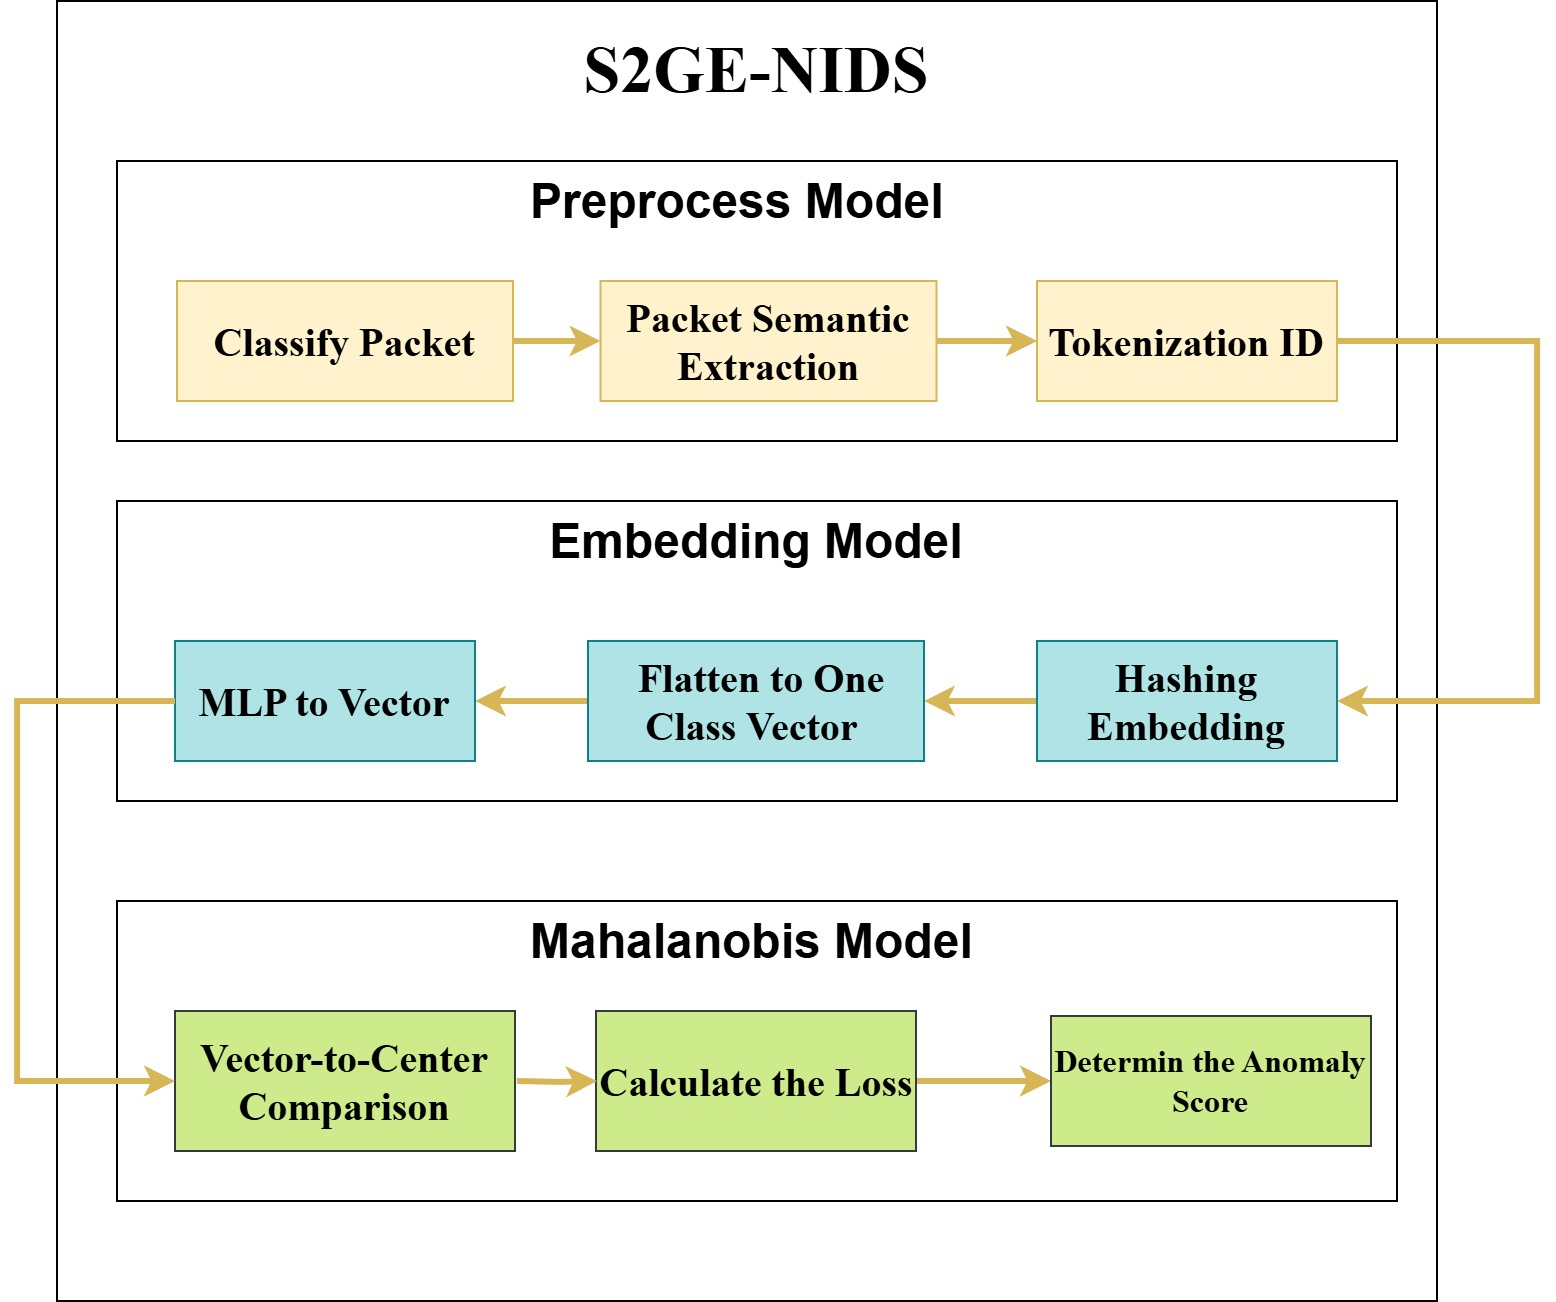
\includegraphics[width = 0.75\textwidth]{image/Flow.jpg}
    \caption{Architecture of S2GE-NIDS}
    \label{fig: Architecture}
\end{figure*}

During the preprocessing stage, relevant features are first extracted from network data packets and transformed into a combination of textual and numerical tokens. To prevent duplication and ensure a more uniform distribution within the embedding space, the model applies the non-encrypted MurmurHash3 function to encode each token.

To further mitigate the risk of hash collisions, a modulo operation is performed on the resulting hash values, which are then used to index into the embedding table. This strategy reduces the likelihood of different tokens being mapped to the same location, thereby enhancing both the accuracy and efficiency of the embedding process.

Next, the individual embedding vectors corresponding to each feature are concatenated into a single one-dimensional vector. This flattened vector is fed into a multi-layer perceptron (MLP) model, which transforms it into a compact semantic representation.

Finally, in the Mahalanobis distance evaluation phase, the semantic vector is compared to a predefined center point in the learned semantic space. If the computed distance exceeds a specified threshold, the sample is flagged as an anomaly. Evaluation metrics such as the F1 score are then used to quantify detection performance.

\subsection{Preprocess Model}
In the preprocessing phase, we will do the following process as data file selection and filtering, feature extraction, and tokenization. These steps are designed to transform raw network traffic into structured representations suitable for semantic embedding and anomaly detection. 

\subsection*{A、Classify Data Packet}

The first step in the preprocessing pipeline involves selecting and filtering the data files to ensure suitability for subsequent analysis. In this study, network traffic is collected and stored in the Comma-Separated Values (CSV) format—a widely adopted and flexible tabular data structure. CSV files are particularly well-suited for structured data representation due to their ease of parsing, compact storage, and seamless integration with mainstream data analysis libraries such as pandas and NumPy in Python.During this stage, only those CSV files containing the required packet-level features are retained, while incomplete, irrelevant, or malformed files are systematically excluded. 

\subsection*{B、Packet Semantic Extraction}

After the data is cleaned and organized, the first step is to extract meaningful features from the network packet data to better capture the characteristics of each packet. For example, we focus on key fields such as Destination Port, Protocol, and SrcIP, which are widely used in previous studies to detect abnormal network behavior  [42]. 
In practice, we use Python tools to read each CSV file and select these important features as the main input for the S2GE-NIDS model. By focusing only on these key values, we can make the data cleaner and easier for the anomaly detection system to use.

\subsection*{C、Tokenization ID}
After the relevant features have been extracted, the next step is to perform tokenization, which converts structured data into a format suitable for semantic embedding. Each data entry consists of multiple fields—such as \texttt{Destination Port}, \texttt{Protocol}, and \texttt{SrcIP}—that represent different aspects of network behavior.

Tokenization is achieved by concatenating each field name with its corresponding value to form a unique string representation. This composite token serves as the semantic unit used in downstream embedding processes. For example, tokens follow the format \textit{"field name + field value"}, as illustrated in Table~\ref{tab:token_example}.

 
\begin{table*}[htbp]
    \centering
    \caption{Example of Tokenized Input Fields} \label{tab:token_example}
    \makebox[\linewidth][c]{
        \renewcommand\arraystretch{1.2}{
            \begin{tabular}{| l | l |}
            \hline
            \textbf{Field Name} & \textbf{Field Value} \\
            \hline
            Destination Port & 80 \\
            Flow Duration & 192.168.1.2 \\
            Protocol Type & TCP \\
            \hline
            \end{tabular}
        }}
    \end{table*}
    


\subsection{Embedding Model}
To mitigate redundancy in text features during the embedding process, we employ a lightweight, non-cryptographic hash function—MurmurHash3. This function ensures that input tokens are more uniformly distributed across the embedding space, thus reducing overrepresentation in specific regions. To further minimize the probability of hash collisions—i.e., multiple tokens being mapped to the same position—we apply a modulo operation to the resulting hash values. This yields a deterministic index used to locate or store each feature vector within a fixed-size embedding table, enhancing both the accuracy and efficiency of the overall embedding process.

Once all relevant token embeddings are retrieved, their vectors are concatenated into a single flattened, one-dimensional feature vector. This unified representation is then fed into a multi-layer perceptron (MLP), which learns high-level semantic abstractions and generates a compact semantic feature vector. The subsequent subsections provide detailed descriptions of the hash embedding mechanism, the flattening procedure, and the structure of the MLP used for semantic encoding.

\subsection*{A、Hash Embedding}
Hash embedding is a lightweight vectorization technique that utilizes non-cryptographic hashing to encode tokenized field-value pairs into fixed-size, trainable embeddings~\cite{weinberger2009feature}. In this study, we adopt the MurmurHash3 algorithm—an efficient and widely used hash function—to map each token to a specific position in the embedding table. Its advantages include fast computation, uniform distribution, and language-independent implementation, which make it well-suited for scalable anomaly detection in IoT environments~\cite{appleby2011murmurhash}.

To determine the target index for each token, we apply a modulo operation to the hash value using the smallest three-digit prime number, 233. This approach distributes tokens more evenly within the embedding space and reduces collision rates. For example, the token generated from the field name \texttt{PORT} may yield a MurmurHash3 value of 4283257230. Applying \texttt{4283257230 mod 233} results in 56. If the associated port number (e.g., 405) is similarly hashed and gives a value with mod 233 result of 7, these indices (row 7, column 56) are used to locate the corresponding vector in the embedding table.

Each embedding vector is initially randomized and refined during training. For instance, an example 8-dimensional vector might be:



\[
[-0.982,\ -0.301,\ -0.555,\ 2.061,\ 0.045,\ -0.618,\ -0.786,\ 0.573]
\]



These vectors are later concatenated and passed to the MLP model for further semantic encoding.




\subsection*{B、Flatten}
Flatten will string the tokenized data into a single vector through the vectors after the embedding column. For example, Destinazation port 405 is [-0.982, -0.301, -0.555, 2.061, 0.045, -0.618, -0.786, 0.573] andXXX經過tokenization變成[-0.024, 0.494, 0.754, -0.78, -1.002, 0.069, -0.52, -1.336] ,XXX [-1.042, -0.116, 0.542, -0.987, 1.001, 0.086, 0.699, -0.903]
[-0.982, -0.301, -0.555, 2.061, 0.045, -0.618, -0.786, 0.573, -0.024, 0.494, 0.754, -0.78, -1.002, 0.069, -0.52, -1.336, -1.042, -0.116, 0.542, -0.987, 1.001, 0.086, 0.699, -0.903]


\subsection*{C、MLP}
After generating semantic embeddings from each tokenized field, the resulting vectors are flattened into a single one-dimensional input vector. This unified semantic representation is then fed into a lightweight \textbf{Multi-Layer Perceptron (MLP)} to learn deeper semantic relationships and perform nonlinear transformation for anomaly detection.

The MLP adopted in this work is composed of an input layer, one or more hidden layers, and an output feature vector. Each layer consists of a fully connected network of neurons activated by the ReLU (Rectified Linear Unit) function, which enables the model to capture non-linear dependencies among input features while maintaining computational efficiency.

To prevent overfitting and enhance generalization, dropout layers are incorporated after each dense layer, and batch normalization is applied to stabilize the training process. The final output of the MLP is a low-dimensional semantic vector projected in a latent space. This vector is subsequently used for statistical anomaly detection based on its distance from a learned semantic center.

Compared to more complex architectures such as transformers or recurrent models, the MLP achieves an optimal balance between \textit{expressiveness, interpretability, and computational efficiency}, making it particularly suitable for deployment in IoT environments with limited resources~\cite{mlp2001universal, 


\subsection{Mahalanobis-Based Semantic Distance Scoring}
In the final stage of the S2GE-NIDS framework, we apply a statistical distance-based method—\textbf{Mahalanobis Distance}—to evaluate whether an observed semantic vector deviates significantly from the expected distribution of normal traffic. This metric is particularly effective for high-dimensional anomaly detection, as it accounts for feature correlations and variance~\cite{de2000mahalanobis}.

Let $\mathbf{x} \in \mathbb{R}^n$ denote the semantic vector output from the MLP, and let $\boldsymbol{\mu}$ and $\boldsymbol{\Sigma}$ represent the mean vector and covariance matrix estimated from a subset of benign (normal) training data. The Mahalanobis distance is defined as:



\[
D_M(\mathbf{x}) = \sqrt{(\mathbf{x} - \boldsymbol{\mu})^T \boldsymbol{\Sigma}^{-1} (\mathbf{x} - \boldsymbol{\mu})}
\]



This formulation enables the model to assess how far a sample deviates from the learned semantic center under multivariate normality assumptions. During inference, if $D_M(\mathbf{x})$ exceeds a predefined threshold $\tau$, the corresponding traffic instance is flagged as an anomaly.

We empirically determine $\tau$ using the distribution of distances in the training set, often by selecting a percentile threshold (e.g., 95th percentile). This thresholding strategy is advantageous in unsupervised or semi-supervised settings, where labeled anomaly samples may be scarce.

The integration of Mahalanobis scoring into our system introduces the benefits of model interpretability and statistical rigor, effectively enhancing the ability to detect subtle but semantically meaningful deviations in IoT network behavior.


\subsection*{A、Vector-to-Center Comparison}
To enhance anomaly detection, S2GE-NIDS introduces a center loss mechanism. During training, all semantic vectors corresponding to "normal" samples are aggregated to calculate a center point  𝑐,

•	Taking into account the variability and correlation of each feature, more accurately detect abnormal samples that are "off-center“

\begin{itemize}
    \item Taking into account the variability and correlation of each feature, we can more accurately detect abnormal samples that are ``off-center''.
\end{itemize}

\begin{equation}
D_M(z) = \sqrt{(z - c)^T \Sigma^{-1} (z - c)}
\label{eq:mahalanobis}
\end{equation}

$z$ is the semantic vector of the input sample, $c$ is the center vector of normal samples, and $\Sigma^{-1}$ is the inverse of the covariance matrix of the training data's embedding vectors.

\subsection*{B、Calculate the Loss}
\begin{itemize}
    \item The loss is defined as:
\end{itemize}

\begin{equation}
\mathcal{L} = \frac{1}{N} \sum_{i=1}^{N} \| z_i - c \|^2 
= \frac{1}{N} \sum_{i=1}^{N} \sum_{j=1}^{d} (z_{ij} - c_j)^2
\label{eq:centerloss}
\end{equation}

$z_i \\in \\mathbb{R}^d$ is the embedding vector obtained after the $i$th input passes through the semantic encoder,  
$c \\in \\mathbb{R}^d$ is the center point vector computed during training, and $N$ is the total number of training samples.


\subsection*{C、Determine the Anomaly Score}






\end{ZhChapter}